\documentclass[10pt]{article}

\usepackage[margin=0.72in]{geometry}
\usepackage[T1]{fontenc}
\usepackage[utf8]{inputenc}
\usepackage{lmodern}
\usepackage{amsmath,amssymb,mathtools}
\usepackage{booktabs,array,longtable,multicol}
\usepackage{enumitem}
\usepackage{siunitx}
\usepackage{xcolor}
\usepackage{hyperref}
\usepackage{tikz,pgfplots,circuitikz}
\usepackage[most]{tcolorbox}
\usetikzlibrary{arrows.meta,positioning,calc,shapes.geometric}
\pgfplotsset{compat=1.18}
\sisetup{per-mode=symbol}
\hypersetup{colorlinks=true,linkcolor=blue!55!black,urlcolor=blue!55!black}
\setlist[itemize]{topsep=2pt,itemsep=2pt,leftmargin=*}
\setlist[enumerate]{topsep=2pt,itemsep=2pt,leftmargin=*}
\renewcommand{\arraystretch}{1.16}
\raggedbottom

\definecolor{GuideBlue}{RGB}{0,74,130}
\definecolor{GuideGreen}{RGB}{231,247,235}
\definecolor{GuideYellow}{RGB}{255,249,226}
\definecolor{GuideRed}{RGB}{255,240,240}
\newtcolorbox{keybox}[1]{enhanced,breakable,colback=blue!4,colframe=GuideBlue,
  title=\textbf{#1},arc=1.5mm,boxrule=0.6pt}
\newtcolorbox{examplebox}[1]{enhanced,breakable,colback=GuideYellow,colframe=orange!70!black,
  title=\textbf{Worked example: #1},arc=1.5mm,boxrule=0.6pt}
\newtcolorbox{cautionbox}[1]{enhanced,breakable,colback=GuideRed,colframe=red!60!black,
  title=\textbf{Caution: #1},arc=1.5mm,boxrule=0.6pt}
\newcommand{\dd}{\mathrm{d}}
\newcommand{\jj}{\mathrm{j}}
\newcommand{\e}{\mathrm{e}}
\newcommand{\rms}{\mathrm{rms}}
\newcommand{\avg}{\mathrm{avg}}
\newcommand{\pwr}{\mathrm{P}}
\newcommand{\phasor}[1]{\underline{#1}}
\newcommand{\abs}[1]{\left|#1\right|}
\newcommand{\degreeC}{^\circ\mathrm{C}}

\title{\textbf{Electrical and Electronics Engineering Basics}\\
\large A focused undergraduate reference: circuits, electronics, machines, digital, controls, measurement, and power}
\author{Study Guide}
\date{\today}

\begin{document}
\maketitle

\begin{abstract}
This reference collects the models and equations used repeatedly in introductory
electrical and electronics engineering. It begins with DC networks and
transients, develops sinusoidal and three-phase analysis, then covers semiconductor
devices, op-amp circuits, transformers and machines, digital electronics, feedback
control, measurement, safety, and introductory power systems. Every worked result
uses the passive sign convention unless stated otherwise: current entering a
positive-labeled terminal means the element absorbs positive power.
\end{abstract}

\begin{keybox}{How to use this guide}
For any circuit: (1) choose voltage polarities and current directions, (2) state
the operating condition---DC steady state, switching transient, or sinusoidal
steady state---and (3) choose a model appropriate to that condition. A negative
answer means the actual direction is opposite the assumed reference direction.
\end{keybox}

\tableofcontents
\newpage

\section{Core Electrical Quantities and DC Networks}

\subsection{Quantities, signs, and power}
Voltage is energy per unit charge, current is charge flow, and resistance opposes
current:
\begin{equation}
  i=\frac{\dd q}{\dd t},\qquad v=\frac{\dd w}{\dd q},\qquad v=Ri,
  \qquad p(t)=v(t)i(t),\qquad w=\int p(t)\,\dd t.
\end{equation}
The SI units are volt (V), ampere (A), ohm ($\Omega$), watt (W), joule (J),
farad (F), henry (H), and hertz (Hz). Power is absorbed when $p>0$ and delivered
when $p<0$ under the passive sign convention.

\subsection{KCL, KVL, and basic combinations}
Kirchhoff's current law (KCL) expresses charge conservation at a node:
\begin{equation} \sum i_{\mathrm{entering}}=\sum i_{\mathrm{leaving}}. \end{equation}
Kirchhoff's voltage law (KVL) expresses energy conservation around a closed loop:
\begin{equation} \sum v_{\mathrm{rises}}=\sum v_{\mathrm{drops}}. \end{equation}
For resistors, series elements share current and parallel elements share voltage:
\begin{equation}
 R_{\mathrm{series}}=\sum_kR_k,\qquad
 \frac{1}{R_{\mathrm{parallel}}}=\sum_k\frac{1}{R_k},\qquad G=\frac1R.
\end{equation}

\begin{figure}[h]
\centering
\begin{circuitikz}[american voltages]
  \draw (0,0) to[battery1,l=$V_s$] (0,3)
        to[R,l=$R_1$,i>^=$i$] (3,3)
        to[R,l=$R_2$,v^>=$v_o$] (3,0) -- (0,0);
  \node at (1.5,-0.45) {Voltage divider};
\end{circuitikz}
\qquad
\begin{circuitikz}[american currents]
  \draw (0,0) to[isource,l=$I_s$] (0,3) -- (3,3)
        to[R,l=$R_1$,i>^=$i_1$] (3,0) -- (0,0);
  \draw (3,3) -- (5,3) to[R,l=$R_2$,i>^=$i_2$] (5,0) -- (3,0);
  \node at (2.5,-0.45) {Current divider};
\end{circuitikz}
\caption{Divider circuits and reference directions.}
\end{figure}

\begin{center}
\begin{tabular}{lll}
\toprule
Network & Useful result & Condition \\
\midrule
Voltage divider & $v_o=V_s\dfrac{R_2}{R_1+R_2}$ & Unloaded output \\
Current divider, two branches & $i_1=I_s\dfrac{R_2}{R_1+R_2}$ & $R_1\parallel R_2$ \\
Power in a resistor & $P=VI=I^2R=V^2/R$ & Passive sign convention \\
\bottomrule
\end{tabular}
\end{center}

\subsection{Network methods}
\textbf{Nodal analysis} solves unknown node voltages with KCL; it is efficient for
current sources and parallel branches. \textbf{Mesh analysis} solves loop currents
with KVL; it is efficient for voltage sources and planar networks. \textbf{Superposition}
finds a linear-circuit response one independent source at a time: replace other
independent voltage sources by shorts and independent current sources by opens.
Dependent sources remain active. Do not superpose power because it is nonlinear.

\subsection{Source transformation, Thevenin, Norton, and maximum power}
A voltage source $V_s$ in series with $R_s$ is equivalent at its terminals to a
current source $I_s=V_s/R_s$ in parallel with $R_s$. Any linear two-terminal
network can be reduced to:
\begin{equation}
  \text{Thevenin: }V_{\mathrm{th}}\text{ in series with }R_{\mathrm{th}},
  \qquad \text{Norton: }I_N\text{ in parallel with }R_N,
\end{equation}
where $R_N=R_{\mathrm{th}}$, $V_{\mathrm{th}}=I_NR_{\mathrm{th}}$, and
$V_{\mathrm{th}}$ is the open-circuit voltage. Find $R_{\mathrm{th}}$ by deactivating
independent sources or by $R_{\mathrm{th}}=V_{\mathrm{test}}/I_{\mathrm{test}}$ when
dependent sources exist. A resistive load receives maximum power at
$R_L=R_{\mathrm{th}}$, with $P_{L,\max}=V_{\mathrm{th}}^2/(4R_{\mathrm{th}})$.

\begin{examplebox}{Loaded voltage divider}
A \SI{12}{V} source feeds $R_1=\SI{2}{k\ohm}$, with $R_2=\SI{4}{k\ohm}$ to
ground. A $\SI{4}{k\ohm}$ load is connected across $R_2$. The load is parallel
with $R_2$, so $R_2\parallel R_L=\SI{2}{k\ohm}$. Therefore
\[
 v_o=\SI{12}{V}\frac{2}{2+2}=\SI{6}{V}.
\]
The unloaded result would be \SI{8}{V}; a real load changes a divider unless its
resistance is much larger than the lower divider resistance.
\end{examplebox}

\section{Capacitors, Inductors, and First-Order Transients}

\subsection{Element laws and DC behavior}
\begin{align}
 i_C&=C\frac{\dd v_C}{\dd t}, & w_C&=\frac12Cv_C^2, & Z_C&=\frac{1}{\jj\omega C},\\
 v_L&=L\frac{\dd i_L}{\dd t}, & w_L&=\frac12Li_L^2, & Z_L&=\jj\omega L.
\end{align}
A capacitor voltage cannot jump without an impulse current:
$v_C(0^+)=v_C(0^-)$. An inductor current cannot jump without an impulse voltage:
$i_L(0^+)=i_L(0^-)$. In a DC steady state, an ideal capacitor is an open circuit
and an ideal inductor is a short circuit. At high frequency, $\abs{Z_C}$ decreases
and $\abs{Z_L}$ increases.

\begin{center}
\begin{tabular}{p{0.19\linewidth}p{0.35\linewidth}p{0.35\linewidth}}
\toprule
 & RC circuit & RL circuit \\
\midrule
State variable & Capacitor voltage $v_C$ & Inductor current $i_L$ \\
Continuity & $v_C(0^+)=v_C(0^-)$ & $i_L(0^+)=i_L(0^-)$ \\
Time constant & $\tau=R_{\mathrm{eq}}C$ & $\tau=L/R_{\mathrm{eq}}$ \\
DC steady state & Capacitor open circuit & Inductor short circuit \\
Natural response & $v_C(t)=V_0\e^{-t/RC}$ & $i_L(t)=I_0\e^{-tR/L}$ \\
\bottomrule
\end{tabular}
\end{center}

\subsection{Universal first-order response}
For a switch at $t=0$, first solve the circuit before switching for the initial
condition, then solve the circuit after switching at $t\to\infty$ for the final
condition. Any first-order state variable has the form
\begin{equation}
 x(t)=x(\infty)+\left[x(0^+)-x(\infty)\right]\e^{-t/\tau},\qquad t\ge0.
\end{equation}
After $5\tau$, the response is within about $0.7\%$ of its final value. A
\textbf{source-free} circuit has no independent sources after switching, so its
stored energy decays exponentially. A step response includes a nonzero final value.

\begin{figure}[h]
\centering
\begin{circuitikz}[american]
  \draw (0,0) to[battery1,l=$V_s$] (0,3) to[closing switch] (2,3)
        to[R,l=$R$] (4,3) to[C,l=$C$,v^>=$v_C$] (4,0) -- (0,0);
  \node at (1,3.4) {$t=0$};
\end{circuitikz}
\qquad
\begin{circuitikz}[american]
  \draw (0,0) to[battery1,l=$V_s$] (0,3) to[closing switch] (2,3)
        to[R,l=$R$] (4,3) to[L,l=$L$,i>^=$i_L$] (4,0) -- (0,0);
  \node at (1,3.4) {$t=0$};
\end{circuitikz}
\caption{RC and RL step-response circuits.}
\end{figure}

\begin{examplebox}{RC charging and RL current rise}
For $V_s=\SI{10}{V}$, $R=\SI{2}{k\ohm}$, and $C=\SI{50}{\micro F}$,
$\tau=RC=\SI{0.10}{s}$. An initially uncharged capacitor charges as
\[
 v_C(t)=10(1-\e^{-t/0.10})\ \mathrm{V}.
\]
At $t=\SI{0.10}{s}$, $v_C=\SI{6.32}{V}$. If instead $L=\SI{0.20}{H}$ and
$R=\SI{10}{\ohm}$, then $\tau=L/R=\SI{0.020}{s}$ and an initially zero
inductor current rises to $i_L(t)=(10/10)(1-\e^{-t/0.020})$ A.
\end{examplebox}

\section{Sinusoidal AC, Phasors, RLC, and Filters}

\subsection{Sinusoids, RMS, and phasors}
For $v(t)=V_m\cos(\omega t+\theta)$, $f=\omega/(2\pi)$ and
$T=1/f$. A sinusoid has $V_{\rms}=V_m/\sqrt2$ and zero average over a full
cycle. The average of a full-wave rectified sine is $2V_m/\pi$. A phasor uses an
RMS magnitude by convention:
\begin{equation}
 v(t)=\sqrt2\,\mathrm{Re}\{\phasor V\e^{\jj\omega t}\},\qquad
 \phasor V=V_{\rms}\angle\theta.
\end{equation}
In phasor form, $\dd/\dd t\rightarrow\jj\omega$ and KCL/KVL still apply.

\subsection{Impedance and phase}
\begin{center}
\begin{tabular}{lllll}
\toprule
Element & Impedance $Z$ & Current versus voltage & Average real power & DC limit \\
\midrule
Resistor & $R$ & In phase & $I_{\rms}^2R$ & $R$ \\
Inductor & $\jj\omega L$ & Current lags $90^\circ$ & 0 ideal & Short \\
Capacitor & $1/(\jj\omega C)$ & Current leads $90^\circ$ & 0 ideal & Open \\
\bottomrule
\end{tabular}
\end{center}
Admittance is $Y=1/Z=G+\jj B$. In a series RLC circuit,
\begin{equation}
 Z=R+\jj\left(\omega L-\frac1{\omega C}\right),\qquad I=V/Z.
\end{equation}
Resonance occurs at $\omega_0=1/\sqrt{LC}$, where the series impedance is
minimum and current is maximum. For a series RLC, $Q=\omega_0L/R$ and the
approximate bandwidth is $\Delta\omega=\omega_0/Q=R/L$.

\subsection{Power in AC circuits}
Let $\phi=\theta_v-\theta_i$. Instantaneous power is $p(t)=v(t)i(t)$;
its average over a cycle is real power:
\begin{equation}
 P=V_{\rms}I_{\rms}\cos\phi,\quad Q=V_{\rms}I_{\rms}\sin\phi,\quad
 \phasor S=P+\jj Q=\phasor V\phasor I^*,\quad \abs S=V_{\rms}I_{\rms}.
\end{equation}
The power factor is $\mathrm{pf}=P/\abs S=\cos\phi$. Inductive loads are
lagging ($Q>0$) and capacitive loads are leading ($Q<0$).

\begin{examplebox}{Series RL power}
A \SI{120}{V_rms}, \SI{60}{Hz} supply feeds $R=\SI{20}{\ohm}$ and
$L=\SI{53.1}{mH}$. Then $X_L=\omega L\approx\SI{20}{\ohm}$,
$Z=20+\jj20=28.3\angle45^\circ\ \Omega$, and $I=4.24\angle-45^\circ$ A.
Thus $P=I^2R=\SI{360}{W}$, $Q=I^2X_L=\SI{360}{var}$, and pf $=0.707$ lagging.
\end{examplebox}

\subsection{Transfer functions and first-order filters}
The transfer function is $H(s)=Y(s)/X(s)$ with zero initial conditions. Replace
$\dd/\dd t$ by $s$ to obtain it from circuit equations; frequency response is
$H(\jj\omega)$. For a resistor-capacitor low-pass with output across $C$:
\begin{equation}
 H_{LP}(s)=\frac{1}{1+sRC},\quad f_c=\frac{1}{2\pi RC},\quad
 \abs{H_{LP}(\jj\omega)}=\frac{1}{\sqrt{1+(\omega RC)^2}}.
\end{equation}
For the high-pass output across $R$:
\begin{equation}
 H_{HP}(s)=\frac{sRC}{1+sRC}.
\end{equation}
At $f_c$, magnitude is $1/\sqrt2$ ($-\SI{3}{dB}$). A first-order magnitude
slope is \SI{20}{dB/decade} beyond its corner: down for low-pass, up for high-pass.

\begin{figure}[h]
\centering
\begin{circuitikz}[american]
  \draw (0,0) to[sV,l=$v_i$] (0,2.5) -- (1,2.5) to[R,l=$R$] (3,2.5)
        to[short,-o] (4,2.5);
  \draw (3,2.5) to[C,l=$C$] (3,0) -- (0,0);
  \node at (4.25,2.5) {$v_o$};
\end{circuitikz}
\qquad
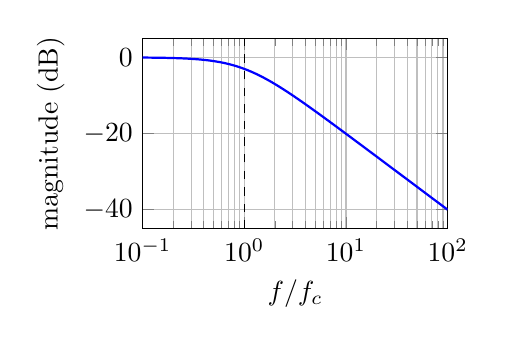
\begin{tikzpicture}
\begin{axis}[width=0.45\linewidth,height=4cm,xmode=log,xmin=.1,xmax=100,
  ymin=-45,ymax=5,xlabel={$f/f_c$},ylabel={magnitude (dB)},grid=both]
\addplot[blue,thick,domain=.1:100,samples=100]{20*log10(1/sqrt(1+x^2))};
\addplot[dashed] coordinates {(1,-45) (1,5)};
\end{axis}
\end{tikzpicture}
\caption{RC low-pass filter and its exact magnitude response.}
\end{figure}

\section{Balanced Three-Phase Circuits and Y-Delta Networks}

\subsection{Three-phase basics}
Balanced phase voltages have equal magnitudes separated by $120^\circ$.
Positive sequence is $a\rightarrow b\rightarrow c$. A balanced load may be
analyzed one phase at a time. Use RMS line-to-line voltage $V_{LL}$ and line
current $I_L$ for total three-phase power:
\begin{equation}
 \phasor S_{3\phi}=\sqrt3\,\phasor V_{LL}\phasor I_L^*,\qquad
 P=\sqrt3V_{LL}I_L\cos\phi,\qquad Q=\sqrt3V_{LL}I_L\sin\phi.
\end{equation}

\begin{center}
\small
\begin{tabular}{p{0.2\linewidth}p{0.34\linewidth}p{0.34\linewidth}}
\toprule
Relationship & Balanced Y (wye/star) load & Balanced Delta load \\
\midrule
Connection & Each impedance phase-to-neutral & Each impedance line-to-line \\
Phase voltage & $V_\phi=V_{LL}/\sqrt3$ & $V_\phi=V_{LL}$ \\
Line/phase current & $I_L=I_\phi$ & $I_L=\sqrt3I_\phi$ \\
Phase current & $I_\phi=V_\phi/Z_\phi$ & $I_\phi=V_\phi/Z_\phi$ \\
Per-phase power & $S_\phi=V_\phi I_\phi^*$ & $S_\phi=V_\phi I_\phi^*$ \\
Total balanced power & $S_{3\phi}=3S_\phi=\sqrt3V_{LL}I_L^*$ & Same result \\
Equal line-current impedance & $Z_Y=Z_\Delta/3$ & $Z_\Delta=3Z_Y$ \\
\bottomrule
\end{tabular}
\end{center}

\begin{figure}[h]
\centering
\begin{circuitikz}[american]
  \draw (0,2) node[left]{$a$} -- (1,2) to[R,l=$Z_a$] (2,1);
  \draw (0,0) node[left]{$b$} -- (1,0) to[R,l_=$Z_b$] (2,1);
  \draw (2,1) to[R,l=$Z_c$] (3,1) node[right]{N};
\end{circuitikz}
\qquad
\begin{circuitikz}[american]
  \draw (0,0) node[left]{$a$} to[R,l=$Z_{ab}$] (2,0) node[right]{$b$}
        to[R,l=$Z_{bc}$] (1,1.8) node[above]{$c$} to[R,l=$Z_{ca}$] (0,0);
\end{circuitikz}
\caption{Wye and delta impedance networks.}
\end{figure}

\subsection{Delta-wye transformation}
For delta impedances $Z_{ab}$, $Z_{bc}$, $Z_{ca}$ and
$\Sigma_\Delta=Z_{ab}+Z_{bc}+Z_{ca}$:
\begin{equation}
 Z_a=\frac{Z_{ab}Z_{ca}}{\Sigma_\Delta},\quad
 Z_b=\frac{Z_{ab}Z_{bc}}{\Sigma_\Delta},\quad
 Z_c=\frac{Z_{bc}Z_{ca}}{\Sigma_\Delta}.
\end{equation}
For wye impedances $Z_a$, $Z_b$, $Z_c$ and
$\Sigma_Y=Z_aZ_b+Z_bZ_c+Z_cZ_a$:
\begin{equation}
 Z_{ab}=\frac{\Sigma_Y}{Z_c},\quad Z_{bc}=\frac{\Sigma_Y}{Z_a},\quad
 Z_{ca}=\frac{\Sigma_Y}{Z_b}.
\end{equation}

\begin{examplebox}{Balanced delta load power}
Three equal $12\angle30^\circ\ \Omega$ impedances form a delta load on a
\SI{208}{V} line-to-line source. Each branch sees \SI{208}{V}, so
$I_\phi=208/12=\SI{17.33}{A}$. The line current magnitude is
$I_L=\sqrt3(17.33)=\SI{30.0}{A}$. With pf $=\cos30^\circ=0.866$ lagging,
\[
 P=\sqrt3(208)(30)(0.866)=\SI{9.36}{kW},\qquad
 Q=\SI{5.40}{kvar}.
\]
\end{examplebox}

\subsection{Power-factor correction}
To improve a lagging load from $\phi_1$ to $\phi_2$ while retaining real power
$P$, add a shunt capacitor supplying
\begin{equation}
 Q_C=P(\tan\phi_1-\tan\phi_2),\qquad C=\frac{Q_C}{\omega V^2}.
\end{equation}
Use phase voltage $V$ for a per-phase capacitor or line-to-line voltage for a
delta-connected capacitor bank. Capacitors reduce source current but do not
reduce the load's real-power demand.

\section{Diodes, BJTs, and MOSFETs}

\subsection{PN junctions and diodes}
A diode conducts strongly in forward bias and blocks current in reverse bias
until breakdown. Common circuit models are ideal ($V_D=0$ when on), constant
drop ($V_D\approx\SI{0.7}{V}$ for silicon), and exponential:
\begin{equation} i_D=I_S\left(\e^{v_D/(nV_T)}-1\right),\qquad V_T\approx\SI{25.9}{mV}\ \text{at }\SI{300}{K}. \end{equation}
A Zener diode is designed for reverse breakdown regulation. A capacitor-filtered
full-wave rectifier has ripple approximately $\Delta V\approx I_{load}/(2fC)$;
use only after confirming capacitor voltage and ripple-current ratings.

\begin{figure}[h]
\centering
\begin{circuitikz}[american]
  \draw (0,0) to[sV,l=$v_s$] (0,3) to[D,l=$D$] (3,3) to[R,l=$R_L$,v^>=$v_o$] (3,0) -- (0,0);
\end{circuitikz}
\qquad
\begin{circuitikz}[american]
  \draw (0,0) to[R,l=$R_s$] (3,0) to[short,-o] (4,0);
  \draw (3,0) to[zD,l=$V_Z$] (3,-2) node[ground]{};
  \draw (0,0) node[left]{$V_{in}$}; \node at (4.3,0) {$V_o$};
\end{circuitikz}
\caption{Half-wave rectifier and Zener shunt regulator.}
\end{figure}

\subsection{BJT and MOSFET essentials}
An NPN BJT operates in cutoff (off), forward active (amplification), and
saturation (switch on). In forward active operation,
\begin{equation} I_C\approx\beta I_B,\qquad I_E=I_C+I_B,\qquad V_{BE}\approx\SI{0.7}{V}. \end{equation}
For switching, choose sufficient base current to force saturation and respect
collector current, $V_{CE}$, power, and switching-speed limits.

An enhancement NMOS is voltage controlled. It is off when $V_{GS}<V_{TH}$,
operates in triode/ohmic region when $V_{DS}<V_{GS}-V_{TH}$, and saturation
when $V_{DS}\ge V_{GS}-V_{TH}$. A basic long-channel saturation model is
\begin{equation} I_D\approx\frac{k}{2}(V_{GS}-V_{TH})^2(1+\lambda V_{DS}). \end{equation}
In a switching NMOS, low $R_{DS(on)}$ minimizes $I^2R$ loss. The insulated gate
draws little DC current but has gate charge: a driver must charge/discharge it
quickly. A MOSFET body diode matters in bridge and inductive-load circuits.

\begin{center}
\small
\begin{tabular}{p{0.2\linewidth}p{0.35\linewidth}p{0.35\linewidth}}
\toprule
Feature & BJT & MOSFET \\
\midrule
Control & Current-driven base-emitter junction & Voltage-driven insulated gate \\
On-state loss & $V_{CE(sat)}I_C$ in saturation & $I_D^2R_{DS(on)}$ \\
Input requirement & Continuous base current & Gate-charge pulses, near-zero DC gate current \\
Strength & Predictable analog gain, low-cost small signal & Fast, efficient switching; high input impedance \\
Key caution & Thermal runaway risk; forced $\beta$ for switching & Gate oxide ESD; body diode and $V_{GS,max}$ \\
\bottomrule
\end{tabular}
\end{center}

\begin{examplebox}{LED resistor and MOSFET switch}
A \SI{5}{V} supply drives a red LED with $V_F=\SI{2}{V}$ at \SI{10}{mA}.
Choose $R=(5-2)/0.010=\SI{300}{\ohm}$; \SI{330}{\ohm} is a common safe value.
For a low-side NMOS switching a \SI{2}{A} load with $R_{DS(on)}=\SI{50}{m\ohm}$,
the approximate conduction loss is $I^2R=2^2(0.05)=\SI{0.20}{W}$. Verify the
data-sheet thermal resistance, voltage rating, gate-drive voltage, and inductive
flyback path before selecting the device.
\end{examplebox}

\section{Operational Amplifiers and Analog Building Blocks}

\subsection{Ideal op-amp model and negative feedback}
For an ideal op-amp, input current is zero, open-loop gain is infinite, and,
with negative feedback in linear operation, $v_+=v_-$. Real devices have finite
gain/bandwidth, input bias and offset, limited common-mode range, finite output
current, finite slew rate, and output swing limited by their supply rails.

\begin{center}
\small
\begin{tabular}{p{0.26\linewidth}p{0.34\linewidth}p{0.28\linewidth}}
\toprule
Circuit & Connection / transfer & Main use \\
\midrule
Voltage follower & $v_o=v_i$ & Buffer; high input, low output impedance \\
Inverting amplifier & $v_o=-(R_f/R_{in})v_i$ & Gain and inversion \\
Non-inverting amplifier & $v_o=(1+R_f/R_g)v_i$ & Gain without inversion \\
Summing amplifier & $v_o=-R_f\sum(v_k/R_k)$ & Weighted addition \\
Difference amplifier & $v_o=(R_2/R_1)(v_2-v_1)$ if ratios match & Subtraction / sensing \\
Transimpedance & $v_o=-i_{in}R_f$ & Photodiode/current sensor \\
Comparator & output saturates high/low & Threshold decision; no linear feedback \\
\bottomrule
\end{tabular}
\end{center}

\begin{figure}[h]
\centering
\begin{circuitikz}[american]
  \draw (0,0) node[op amp,anchor=-] (opamp) {};
  \draw (-2,-.5) to[R,l=$R_{in}$] (opamp.-);
  \draw (opamp.+) -- ++(-.6,0) node[ground]{};
  \draw (opamp.out) -- ++(1,0) node[right]{$v_o$};
  \draw (opamp.out) ++(.5,0) |- (0,1.5) to[R,l=$R_f$] (opamp.-);
  \node[left] at (-2,-.5) {$v_i$};
\end{circuitikz}
\caption{Inverting op-amp amplifier under negative feedback.}
\end{figure}

\begin{examplebox}{Non-inverting gain design}
Design a non-inverting amplifier with gain 11. Since $A_v=1+R_f/R_g$, choose
$R_g=\SI{10}{k\ohm}$ and $R_f=\SI{100}{k\ohm}$. A \SI{0.20}{V} input ideally
produces \SI{2.20}{V}. Confirm that this output is inside the chosen op-amp's
supply and output-swing limits, and that the required closed-loop bandwidth
exceeds the signal frequency.
\end{examplebox}

\section{Transformers, Machines, and Introductory Power Systems}

\subsection{Ideal transformer and practical losses}
For an ideal transformer with turns ratio $a=N_p/N_s$:
\begin{equation}
 \frac{V_p}{V_s}=a,\qquad \frac{I_p}{I_s}=\frac1a,\qquad
 Z_{\mathrm{seen\ at\ primary}}=a^2Z_L,\qquad P_p=P_s.
\end{equation}
It requires changing flux, so it does not continuously transform DC. Real
transformers have copper loss ($I^2R$), core hysteresis/eddy-current loss,
leakage reactance, magnetizing current, regulation, and insulation limits.

\subsection{Machine fundamentals}
\begin{center}
\small
\begin{tabular}{p{0.22\linewidth}p{0.3\linewidth}p{0.36\linewidth}}
\toprule
Machine & Principle & Key relation / feature \\
\midrule
DC machine & Commutator maintains unidirectional torque & $E\propto\Phi\omega$, $T\propto\Phi I_a$ \\
Induction motor & Rotor current induced by rotating stator field & $n_s=120f/P$, $s=(n_s-n_r)/n_s$ \\
Synchronous machine & Rotor field locks to rotating stator field & $n_r=n_s=120f/P$ in steady operation \\
\bottomrule
\end{tabular}
\end{center}
An induction motor must run below synchronous speed in motoring operation so
that slip induces rotor current. Increasing mechanical load generally increases
slip and rotor current. Motor starting current can be large; protection and
starting method matter.

\subsection{Power-system essentials}
A power system has generation, transformers, transmission, distribution,
switchgear, loads, grounding, and protection. A one-line diagram represents a
balanced three-phase network with one conductor. Per-unit normalizes quantities:
\begin{equation}
 Z_{base}=\frac{V_{LL,base}^2}{S_{3\phi,base}},\qquad
 I_{base}=\frac{S_{3\phi,base}}{\sqrt3V_{LL,base}},\qquad x_{pu}=\frac{x}{x_{base}}.
\end{equation}
Circuit breakers interrupt fault current; fuses open on overcurrent; relays
sense conditions and command breakers. Grounding provides a defined reference
and a fault-current path; it does not make energized conductors safe to touch.

\begin{examplebox}{Transformer impedance reflection}
A \SI{120}{V}:\SI{24}{V} ideal transformer supplies a \SI{6}{\ohm} load.
The primary-to-secondary ratio is $a=120/24=5$, so the primary sees
$Z_{in}=a^2Z_L=25(6)=\SI{150}{\ohm}$. The secondary current is
$24/6=\SI{4}{A}$ and the primary current is $4/5=\SI{0.8}{A}$; both sides
carry \SI{96}{W} ideally.
\end{examplebox}

\section{Digital Electronics and Data Conversion}

\subsection{Logic fundamentals}
Logic signals represent 0 and 1 within guaranteed voltage ranges. Essential
Boolean identities include $\overline{\overline A}=A$,
$A+\overline A=1$, $A\overline A=0$, and De Morgan's laws:
\begin{equation} \overline{AB}=\overline A+\overline B,\qquad \overline{A+B}=\overline A\,\overline B. \end{equation}
AND, OR, and NOT are universal building blocks; NAND and NOR alone can implement
any Boolean function. XOR is 1 when inputs differ. Combinational logic depends
only on current inputs; sequential logic also stores state.

\begin{center}
\begin{tabular}{llll}
\toprule
Element & Function & Clocked? & Typical use \\
\midrule
Multiplexer & Select one input & No & Data routing \\
Decoder & Activate one output from binary code & No & Address selection \\
D flip-flop & Store $D$ at active clock edge & Yes & Register / synchronizer \\
Counter & Advance stored binary state & Yes & Timing / frequency division \\
Register & Group of flip-flops & Yes & Multi-bit storage \\
\bottomrule
\end{tabular}
\end{center}

\subsection{ADC, DAC, sampling, and resolution}
An $N$-bit ADC has $2^N$ codes; for input range $V_{FS}$, its ideal LSB size is
approximately $V_{FS}/2^N$. To avoid aliasing for a band-limited signal, sample
above twice its highest frequency: $f_s>2f_{max}$, and use an anti-alias low-pass
filter before the ADC. A DAC converts code to analog voltage; its reference
accuracy, integral/differential nonlinearity, settling time, and output drive
matter in practice.

\begin{examplebox}{ADC resolution}
A 12-bit ADC spans \SI{0}{V} to \SI{3.3}{V}. Its ideal step size is
$3.3/2^{12}=\SI{0.806}{mV}$ per count. The quantization uncertainty is commonly
modeled as about $\pm0.5$ LSB, before reference, offset, gain, noise, and
nonlinearity errors are included.
\end{examplebox}

\section{Feedback Control Fundamentals}

\subsection{Transfer functions, poles, and feedback}
For an LTI system, $G(s)=Y(s)/U(s)$ under zero initial conditions. A pole is a
root of the denominator and a zero is a root of the numerator. With negative
feedback $H(s)$, the closed-loop transfer function is
\begin{equation} T(s)=\frac{G(s)}{1+G(s)H(s)}. \end{equation}
Negative feedback can reduce sensitivity and improve disturbance rejection, but
excess phase lag can make the loop oscillate. A stable continuous-time system
has all closed-loop poles in the left half of the $s$ plane.

\subsection{First-order response and PID intuition}
A first-order plant $G(s)=K/(\tau s+1)$ has time response
$y(t)=K(1-\e^{-t/\tau})u(t)$ for a unit step. The $10$--$90\%$ rise time is
about $2.2\tau$. Proportional control responds to current error, integral control
removes constant steady-state error, and derivative action anticipates changing
error but amplifies noise:
\begin{equation} C(s)=K_p+\frac{K_i}{s}+K_ds. \end{equation}
Gain margin and phase margin measure distance from instability in frequency
response. Saturation requires anti-windup when integral action is used.

\section{Measurement, Grounding, and Electrical Safety}

\subsection{Making trustworthy measurements}
\begin{center}
\small
\begin{tabular}{p{0.23\linewidth}p{0.34\linewidth}p{0.31\linewidth}}
\toprule
Instrument & Strength & Main limitation / check \\
\midrule
Digital multimeter & Accurate DC/low-frequency voltage, current, resistance & Burden voltage in current mode; input impedance \\
Oscilloscope & Time-domain waveform, transients, noise & Probe rating, bandwidth, sampling, earth-referenced ground clip \\
Current probe & Nonintrusive current waveform & Range, bandwidth, offset/degauss \\
LCR meter & Component value and loss at stated frequency & Test frequency and fixture parasitics \\
\bottomrule
\end{tabular}
\end{center}
Bandwidth must exceed the signal content; a rule of thumb for a single-pole
instrument is $t_r\approx0.35/BW$. Use a $10\times$ oscilloscope probe when
its reduced loading and higher voltage rating are appropriate, and compensate it
before accurate fast-edge measurement. Report uncertainty from instrument
specification, calibration, repeatability, and setup effects rather than only
display digits.

\subsection{Grounding and safety}
Protective earth (PE) bonds exposed conductive enclosures to reduce touch-voltage
hazard and encourage fault current to clear protection. Signal ground is a circuit
reference; it may be tied to earth at a deliberate point. Avoid accidental ground
loops and never clip an earth-referenced oscilloscope ground lead to a floating
high-side node unless the measurement arrangement is designed for it. Use a
differential probe or isolated measurement system when required.

\begin{cautionbox}{Safe work is a design requirement}
De-energize before changing wiring when possible. Apply lockout/tagout, verify
absence of voltage with a rated meter, use equipment with adequate voltage and
fault-category ratings, and inspect leads, fuses, and insulation. Treat stored
energy in capacitors, rotating equipment, batteries, and inductors as hazardous.
Follow the applicable site procedure and local electrical-safety standard; this
guide is not a substitute for them.
\end{cautionbox}

\section{Formula Review}
\begin{multicols}{2}
\textbf{DC:} $V=IR$; $P=VI=I^2R=V^2/R$; $R_s=\sum R$;
$1/R_p=\sum1/R$; $V_o=V_sR_2/(R_1+R_2)$; $R_L=R_{th}$ for maximum resistive
power.

\textbf{Energy and transients:} $w_C=CV^2/2$; $w_L=LI^2/2$;
$i_C=C\dd v/\dd t$; $v_L=L\dd i/\dd t$; $\tau_{RC}=RC$;
$\tau_{RL}=L/R$; $x=x_\infty+(x_0-x_\infty)\e^{-t/\tau}$.

\textbf{AC:} $V_{rms}=V_m/\sqrt2$; $Z_R=R$; $Z_L=\jj\omega L$;
$Z_C=1/(\jj\omega C)$; $S=VI^*=P+\jj Q$; $P=VI\cos\phi$;
$Q=VI\sin\phi$; pf $=\cos\phi$.

\textbf{Filters and resonance:} $H_{LP}=1/(1+sRC)$;
$H_{HP}=sRC/(1+sRC)$; $f_c=1/(2\pi RC)$; $\omega_0=1/\sqrt{LC}$.

\textbf{Three phase:} $S_{3\phi}=\sqrt3V_{LL}I_L^*$;
$P=\sqrt3V_{LL}I_L\cos\phi$; Y: $V_L=\sqrt3V_\phi$, $I_L=I_\phi$;
Delta: $V_L=V_\phi$, $I_L=\sqrt3I_\phi$.

\textbf{Devices:} $I_C\approx\beta I_B$; $I_D\approx k(V_{GS}-V_{TH})^2/2$;
$A_{inv}=-R_f/R_{in}$; $A_{noninv}=1+R_f/R_g$.

\textbf{Transformer and machines:} $V_p/V_s=N_p/N_s$;
$Z_p=a^2Z_s$; $n_s=120f/P$; $s=(n_s-n_r)/n_s$.

\textbf{Digital and control:} LSB $\approx V_{FS}/2^N$; $f_s>2f_{max}$;
$T=G/(1+GH)$; $C_{PID}=K_p+K_i/s+K_ds$.
\end{multicols}

\section{Mixed Practice Problems with Answers}
\begin{enumerate}
  \item A \SI{24}{V} source drives series \SI{3}{\ohm} and \SI{9}{\ohm}
  resistors. Find current, voltage across \SI{9}{\ohm}, and its power.
  \item An initially charged \SI{10}{\micro F} capacitor at \SI{5}{V} discharges
  through \SI{100}{k\ohm}. Write $v_C(t)$ and find $v_C$ at one time constant.
  \item A \SI{100}{V_rms} supply feeds a \SI{25}{\ohm} resistor. Find average
  power and peak current.
  \item A balanced Y load has $Z_\phi=8+\jj6\ \Omega$ and is supplied by
  \SI{208}{V} line-to-line. Find $I_L$ magnitude and total real power.
  \item Find the inverting-op-amp output for $R_{in}=\SI{5}{k\ohm}$,
  $R_f=\SI{50}{k\ohm}$, and $v_i=\SI{0.30}{V}$.
  \item A four-pole induction motor operates from \SI{60}{Hz} and runs at
  \SI{1740}{rpm}. Find synchronous speed and slip.
\end{enumerate}

\begin{keybox}{Answers}
1. $I=24/(3+9)=\SI{2}{A}$; $V_{9\Omega}=\SI{18}{V}$; $P_{9\Omega}=18(2)=\SI{36}{W}$.

2. $\tau=RC=(100\,000)(10\times10^{-6})=\SI{1}{s}$ and
$v_C(t)=5\e^{-t}\ \mathrm{V}$; at $t=\tau$, $v_C=\SI{1.84}{V}$.

3. $P=V^2/R=100^2/25=\SI{400}{W}$; $I_{rms}=\SI{4}{A}$ and
$I_{peak}=4\sqrt2=\SI{5.66}{A}$.

4. $\abs{Z}=\SI{10}{\ohm}$, $V_\phi=208/\sqrt3=\SI{120}{V}$,
$I_L=I_\phi=120/10=\SI{12}{A}$. With pf $=8/10=0.8$,
$P=\sqrt3(208)(12)(0.8)=\SI{3.46}{kW}$.

5. $v_o=-(50/5)(0.30)=\SI{-3.0}{V}$, provided the supply rails permit it.

6. $n_s=120(60)/4=\SI{1800}{rpm}$ and $s=(1800-1740)/1800=0.0333$, or $3.33\%$.
\end{keybox}

\end{document}